\section{Post-Hoc Hardening Evidence}\label{app:g7}

Everything in this appendix was produced \emph{after} the pre-registered
analysis was frozen, as part of an audit-and-hardening pass. None of it
alters any pre-registered number; all comparisons are internal to this
appendix (block self-containment, \Cref{app:design}).

\subsection{A nonlinear check of Proposition~1}\label{app:g7-mlp}

The structural half of \Cref{prop:deficiency}---that the composed forecast
\Cref{eq:equivariance} is additively separable in the window mean with unit
slope---holds for an arbitrary backbone and needs no check. What is specific
to linear classes is the \emph{quantification}, \Cref{eq:prop1,eq:prop1b}. To
probe whether that geometry survives nonlinearity, we train an identical
two-hidden-layer MLP ($128\times128$, ReLU) under the interaction DGP of
\Cref{sec:theory} in three arms that differ only in the normalization
constraint (\rawm{}, RevIN-style mean removal and restoration, \cnm{}-style
covariate restoration), at $\lambda \in \{0.4, 0.8\}$ with ten seeds, and
measure excess risk over the analytic Bayes predictor.
\Cref{fig:mlpdemo} shows the result: the RevIN-constrained arm cannot go
below the class floor $\kappa^2\,\var(\bar y \mid g)\,\var(g)$ (its mean
sits above the floor by at least $16$ standard errors of the mean at both
$\lambda$), while the unconstrained and covariate-restored arms sit roughly
a factor of twenty below it. That floor is \Cref{eq:prop1c} evaluated at
this configuration: the demo fixes $a = 1$, at which the pinned-slope term
vanishes identically and the whole irreducible excess is the interaction
term $\kappa^2 \var(g)\var(\bar y)(1-\varrho^2) = \kappa^2\var(g)\var(\bar
y \mid g)$. Earlier versions of this appendix carried the constant as
provisional and configurable pending a derivation; Step~7 of
\Cref{app:proofs} supplies it, so the demonstration now serves as a
nonlinear \emph{confirmation} of \Cref{eq:prop1c} rather than a measurement
against a guessed scale. It is also the cleanest illustration of the
proposition's division of labour: because $a=1$ here, nothing in this
figure is attributable to the pinned slope, and the entire gap between the
RevIN arm and the unconstrained arm is the interaction cost that only the
constrained class still pays.

\begin{figure}[htbp]
\centering
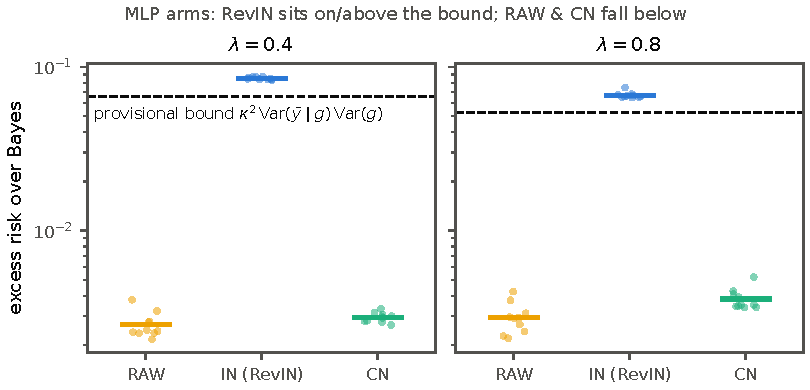
\includegraphics[width=.85\textwidth]{figures/figG_prop1_mlp.pdf}
\caption{Nonlinear check of Proposition~1. Excess risk over the Bayes
predictor for an identical MLP backbone under three normalization
constraints (ten seeds; dots are seeds, bars are means; dashed line is the
provisional RevIN-class floor $\kappa^2\,\var(\bar y \mid g)\,\var(g)$).
The RevIN-constrained arm is pinned above the floor at both $\lambda$;
the unconstrained (\rawm{}) and covariate-restored (\cnm{}) arms are not.}
\label{fig:mlpdemo}
\end{figure}

\subsection{Classical and diagnostic baselines (Block~E)}\label{app:g7-blocke}

\Cref{tab:baselines} adds five reference arms on all eight datasets:
seasonal naive, hour-of-day/day-of-week climatology, the CondNorm first
stage used \emph{alone} as a forecaster, a classical dynamic-regression
stand-in (ridge on lagged target plus target-time covariates, direct
multi-step), and the published-default \texttt{revin\_all} ablation with
its in-block comparators. Three observations. First, on the
exogenously-driven group the first stage alone is already competitive with
the full CondNorm pipeline (e.g., Jeju Wind $0.294$ vs.\ $0.307$;
GEFCom-Wind $0.156$ vs.\ $0.180$): most of conditional normalization's
value on these series is the covariate-to-level map itself, with the
backbone adding shape refinement --- and the same arm collapses on the
standard group (ETTh2 $3.37$), exactly as the boundary predicts. Second,
dynamic regression is competitive on wind ($0.285$ on Jeju) but loses
badly on the nonlinear temperature--load relation ($0.371$ vs.\ $0.108$),
supporting the nonlinear first stage. Third, \texttt{revin\_all}
(window-normalizing covariate channels as published defaults do) stays
within $\pm 0.05$ MSE of target-only normalization on seven of the eight
datasets --- significantly better on one (GEFCom-Wind), significantly
worse on two (Electricity, GEFCom-Load), within seed-level noise on the
remaining four --- but diverges catastrophically on GEFCom-Solar (MSE in
the hundreds at $h=336$, all seeds): an intermittent precipitation
covariate has window standard deviations down to $4\times10^{-6}$ ---
$1/800$ of its global scale --- so window normalization amplifies it
explosively. This is a reproducible
failure case for the published default and the reason our protocol
normalizes the target channel only (\Cref{app:design}).

\begin{table}[htbp]
\centering
\caption{Block~E baselines and ablation (post-hoc hardening block; not
pre-registered): test MSE (global z-score scale; dataset mean over horizons
and seeds). \emph{f/s only} = CondNorm first stage used alone;
\emph{dynreg} = ridge dynamic-regression stand-in; \emph{revin\_all} =
instance normalization applied to covariate channels as well (published
default), with its in-block linmix comparators. \textbf{Bold}: lowest MSE
per row. Self-contained block; no cross-block comparison.}
\label{tab:baselines}
\scriptsize
\setlength{\tabcolsep}{4pt}
\begin{tabular}{@{}lrrrrrrrr@{}}
\toprule
Dataset & s.naive & climat. & f/s only & dynreg & revin\_all & linmix\,\rawm & linmix\,RevIN & linmix\,\cnm \\
\midrule
Jeju Wind    & 1.627 & 1.032 & 0.294 & \textbf{0.285} & 0.349 & 0.344 & 0.367 & 0.307 \\
GEFCom-Wind  & 1.988 & 1.231 & \textbf{0.156} & 0.171 & 0.275 & 0.265 & 0.327 & 0.180 \\
GEFCom-Load  & 0.686 & 1.190 & 0.136 & 0.371 & 0.409 & 0.358 & 0.381 & \textbf{0.108} \\
GEFCom-Solar & 0.333 & 0.203 & \textbf{0.057} & 0.141 & 316.0 & 0.159 & 0.162 & 0.064 \\
ETTh1        & 0.670 & 0.883 & 1.403 & 0.479 & 0.396 & 0.397 & \textbf{0.391} & 2.993 \\
ETTh2        & 0.577 & 3.128 & 3.367 & 0.892 & 0.272 & 0.361 & \textbf{0.270} & 7.392 \\
Weather      & 0.338 & 0.688 & 0.648 & \textbf{0.181} & 0.183 & 0.185 & 0.182 & 1.069 \\
Electricity  & 0.217 & 0.389 & 0.322 & 0.199 & 0.199 & 0.205 & \textbf{0.148} & 0.175 \\
\bottomrule
\end{tabular}
\end{table}

\subsection{Probabilistic robustness (Block~F)}\label{app:g7-blockf}

We re-ran the boundary comparison with quantile forecasting: an RLinear
backbone with a nine-quantile pinball head (Block-A capacities and
lookbacks; all five arms, per-quantile denormalization, non-crossing by
sorting) and a LightGBM quantile backbone (levels $\{0.1,0.5,0.9\}$; arms
as in Block~A). \Cref{tab:prob} reports mean pinball loss and empirical
80\% coverage. The boundary persists in full: CondNorm attains the lowest
pinball in $11/11$ exogenous (dataset,\,$h$) cells on \emph{both}
backbones (mean pinball $0.106$ vs.\ RevIN's $0.197$ on the linear
backbone, a $46\%$ improvement), and the ordering reverses on the standard
group exactly as in Block~A. The relative gap is smaller than under
squared error, as expected when moving from a squared to a
$1$-homogeneous loss. Calibration is the one metric where CondNorm does
not dominate: its 80\% intervals cover $0.60$ on the exogenous group
against RevIN's $0.82$ (nominal $0.80$), with the miscoverage split
roughly evenly between the two tails ($P(y \le q_{0.1}) = 0.19$ vs.\
nominal $0.10$; $P(y > q_{0.9}) = 0.21$ vs.\ nominal $0.10$) --- the
intervals are under-dispersed on both sides. Sharp but symmetrically
under-covered intervals are the probabilistic signature of an unpropagated
variance term ($\sest$ in \Cref{sec:theory}); propagating first-stage
uncertainty into the quantile spread is a natural extension we leave to
future work.

\begin{table}[htbp]
\centering
\caption{Block~F probabilistic robustness (post-hoc hardening block; not
pre-registered): mean pinball loss (empirical 80\% coverage in
parentheses; nominal $0.80$), dataset mean over horizons and seeds. \textbf{Bold}: lowest pinball per row within the backbone.
LightGBM SAN/FAN are structurally N/A as in Block~A; \emph{winz} is the
window z-normalization arm. CRPS approximations preserve the pinball
ordering and are omitted.}
\label{tab:prob}
\scriptsize
\setlength{\tabcolsep}{2.2pt}
\begin{tabular}{@{}lccccc|ccc@{}}
\toprule
 & \multicolumn{5}{c|}{RLinear-Q (9 quantiles)} & \multicolumn{3}{c}{LightGBM-Q ($\{0.1,0.5,0.9\}$)} \\
Dataset & \rawm & RevIN & SAN & FAN & \cnm & \rawm & winz & \cnm \\
\midrule
Jeju Wind    & .223 (.79) & .228 (.80) & .237 (.73) & .284 (.39) & \textbf{.165} (.58) & .182 (.68) & .186 (.71) & \textbf{.134} (.64) \\
GEFCom-Wind  & .320 (.76) & .313 (.79) & .320 (.57) & .431 (.19) & \textbf{.135} (.50) & .257 (.68) & .244 (.71) & \textbf{.105} (.60) \\
GEFCom-Load  & .162 (.83) & .165 (.80) & .167 (.78) & .173 (.75) & \textbf{.085} (.66) & .136 (.74) & .132 (.75) & \textbf{.073} (.65) \\
GEFCom-Solar & .092 (.89) & .092 (.89) & .101 (.84) & .108 (.78) & \textbf{.058} (.65) & .062 (.84) & .066 (.79) & \textbf{.044} (.71) \\
\midrule
ETTh1        & .163 (.79) & \textbf{.160} (.82) & .166 (.73) & .178 (.66) & .604 (.14) & .125 (.77) & \textbf{.122} (.73) & .354 (.38) \\
ETTh2        & .146 (.78) & \textbf{.136} (.74) & .139 (.68) & .155 (.66) & 1.126 (.03) & .168 (.70) & \textbf{.112} (.71) & .616 (.17) \\
Weather      & .096 (.87) & \textbf{.087} (.73) & .089 (.70) & .094 (.86) & .245 (.45) & .070 (.85) & \textbf{.067} (.76) & .200 (.49) \\
Electricity  & .102 (.83) & \textbf{.100} (.82) & .102 (.78) & .101 (.81) & .110 (.65) & .077 (.80) & \textbf{.076} (.79) & .092 (.71) \\
\bottomrule
\end{tabular}
\end{table}

\subsection{Supporting inference for the LPS values}\label{app:g7-lpsinf}

\Cref{tab:lpsinf} adds three post-hoc inferential quantities to the
pre-registered LPS values, all computed under the identical LPS protocol:
a permutation $p$-value against stride-preserving circular shifts of the
covariates (with a season-aligned variant restricting shifts to whole
weeks), a moving-block bootstrap 90\% interval, and a rough plug-in
estimate $\hat{\lambda}^{*}$ of the crossover from measurable quantities.
The exogenous group is uniformly significant ($p \le .008$) with intervals
above $\tau$; the standard group is uniformly compatible with the null.
The plug-in $\hat{\lambda}^{*}$ ordering agrees with the realized winner
on all eight datasets (negative values --- CN dominant at every $\lambda$
--- for the wind datasets; values above one --- IN dominant --- for the
standard group). Electricity is the boundary case on every diagnostic at
once ($\lps=.283$, $p=.058$, $\hat{\lambda}^{*}=1.35$, realized gap
$-0.027$), consistent with its pre-registered lowest-confidence flag.
Bootstrap intervals for negative-LPS series are biased upward (block
resampling dilutes the across-fold drift that produces negative
out-of-sample $R^2$), so the permutation $p$-value is the informative
quantity there.

\begin{table}[htbp]
\centering
\caption{Post-hoc inference for the pre-registered LPS values (identical
protocol: $w=96$, LightGBM first stage, expanding chronological CV).
$p_{\mathrm{perm}}$: circular-shift permutation ($B \le 999$, exact where
enumerable); aligned: shifts restricted to whole weeks; CI: moving-block
bootstrap, 90\%; $\hat{\lambda}^{*}$: plug-in crossover estimate at
$h=96$ (negative $\Rightarrow$ CN dominates all $\lambda$;
$>1 \Rightarrow$ IN dominates). The decision rule remains the
pre-registered $\lps \ge \tau$.}
\label{tab:lpsinf}
\small
\begin{tabular}{@{}lrrrrr@{}}
\toprule
Dataset & $\lps$ & $p_{\mathrm{perm}}$ & aligned & 90\% CI & $\hat{\lambda}^{*}$ \\
\midrule
Jeju Wind    & $.745$  & $.006$ & $.039$ & $[.76,\,.88]$ & $-0.20$ \\
GEFCom-Wind  & $.744$  & $.008$ & $.059$ & $[.70,\,.85]$ & $-0.51$ \\
GEFCom-Load  & $.894$  & $.002$ & $.011$ & $[.90,\,.95]$ & $0.68$ \\
GEFCom-Solar & $.875$  & $.005$ & $.035$ & $[.88,\,.95]$ & $0.09$ \\
ETTh1        & $-.717$ & $.39$  & $.38$  & $[-.02,\,.40]$ & $2.26$ \\
ETTh2        & $-.205$ & $.19$  & $.19$  & $[-.29,\,.42]$ & $2.90$ \\
Weather      & $.110$  & $.36$  & $.41$  & $[-.22,\,.66]$ & $1.02$ \\
Electricity  & $.283$  & $.058$ & $.075$ & $[.38,\,.57]$ & $1.35$ \\
\bottomrule
\end{tabular}
\end{table}
